\documentclass[a4paper]{article}
\usepackage{graphicx}
\usepackage{fullpage}

\title{{RELACS: Reliable Estimator of Local Antagonizing and Counterproductive Sounds}}
\author{Steven Bosch \and Luuk Boulogne \and Pim van der Meulen \and Xeryus Stokkel  \and Rogier de Weert}

\begin{document}

\maketitle

\section{Product purpose}

\subsection{Problem}
Stress is arguably the biggest problem of our society nowadays. It can be very harmful to the health of the individual, as stress can cause problems in both mental and physical health. The effects of living a stressful life can include a reduced urge in reproduction, as well as lowered productivity during work. Throughout the years, many methods have been devised to decrease stress and increase relaxation. The system described onward does not decrease stress or increases relaxation directly, but rather attends the user to the influence of stress-inducing sounds in the environment of the user. When the user is more aware of stressful sounds in its sound environment (also called soundscape) he or she could change or avoid this environment, which might decrease their stress-level.

\subsection{Target group}
Since stress can be experienced by anyone, we did not feel like limiting our product to a specific target audience. We could say that our user group consists of students, people working in an office, construction workers, and the elderly. 
The current version of our product is aimed at an English-speaking audience, although in future versions we hope to increase our user-count with a wider selection of languages. 

\subsection{Improvements}
We aim to improve the user awareness of the stress level in their surroundings.
By showing users that some of the sounds present in their environment are stress-inducing, we want to improve the awareness of the importance of sound in order to create or find a relaxed environment. 
We think that a relaxed environment would benefit a person, as productivity is higher when stress is lower.

\section{Product description}
In the next chapter the complete technical specifications can be found, followed by a performance analysis and a user manual. 
But first a simple representation of the working of RELACS is given. RELACS is a simple tool to see how stressful a sound-sample is. 
When a processed recording of 30 seconds is presented to the tool, it calculates the overall percentage of stressfulness of the sample and shows where in the sample the stressful sounds are located. 
Basically what RELACS does is: sound in, stress analysis out.

A processed recording means that a recording (.wav-file) should first be processed to a cochleogram (as in a .hdf5 file) before it can be presented to RELACS. The system then cuts the sample in windows of each 128

\section{Technical specifications}


\section{Performance analysis}
This section gives an overview of the performance analysis, discussing the strengths, weaknesses, opportunities and threats of our application.

\subsection{Internal factors}
\subsubsection{Strengths}
Perhaps the main strength of RELACS is that it tries to address a highly significant and common problem in society. Stress is one of the most dire problems in the modern western world. Not only does it effect the happiness of many, it also has significant consequences for public health and with it for state and private finances. It is therefore imperative that causes of stress are identified and prevented. Sound may be a relatively `small' cause for stress, but the contribution of RELACS extends beyond just making people aware of stress-inducing sounds in their environment. It also makes them aware of the fact that they can actively work to decrease their stress level. If the cause is not in their sound environment, the application might have triggered them to remove or reduce other stress-inducing aspects in their live.

Aside from this last aspect, RELACS itself of course only focuses on sound. Its main strength in that respect is its innovative property. There is no other application (of which we are aware) that does anything on stress-inducing sound recognition. There are applications that try to counter stress by producing `relaxing' or `anti-stress' sounds. But, while these application may help reduce stress in certain situation, it is often not the absence of relaxing sounds that causes stress, but the presence of stress-inducing sounds. This is where our application comes in, making it potentially more effective than the other available stress and sound related applications.

Another strength of RELACS is that it provides a more or less objective assessment of the stressfulness of the sounds in the environment. The application bases its assessment on the input of multiple users (we could add user feedback to make this \textit{all} of the users). As a result, the sounds it classifies as stressful are likely to be found stressful by a majority of the people. It could therefore be used in objective stressfulness measurements, which could be useful, for example in the case of an employee trying to convince his superiors that the work floor sound environment induces stress. Of course there is the issue that some users would not find certain sounds stressful, while the application indicates them as such. While our current application cannot deal with that issue yet, user customization could be added to counter this issue. A user could then specify whether it would find certain sounds stressful or not, and the system would accommodate for those preferences.

Finally, when we look at the technical aspect of RELACS, we can distinguish a strength in its flexibility. Because of its adaptive back-end, user input could be very well accounted for and used to improve the accuracy of its classifications. The classifiers would only have to be retrained with the new data. You could, for example, release an update to the application every month, until the amount of data is such that changes in classification would not happen anymore. Or, in the light of user customization as discussed above, customized classifiers could be trained which would classify sounds specifically for that user.

\subsubsection{Weaknesses}
Although RELACS has several strengths, unfortunately the application poses a number of weaknesses as well.

The first weakness starts where the last strength left of. Its flexibility and user customization possibilities are not without consequence. Training our classifier, for example, is something that could never happen client side, since it takes an average pc or laptop about twelve to fourteen hours of time (we dare not say what would happen on a phone). This means that we would have no other choice than doing this server-side. We would thus need a lot of processing power and storage space if every user would require a customized classifier, and of course users do not like waiting for their customized app for half a day. So implementing user customization would require more thinking.

A major weakness of the existing application (without user customization) is its recognition rate. While we reach a reasonable rate (around 80\%), it is still far from human level. This is due to the nature of stress-inducing sounds: while the bulk of it has some clear characteristics, such as loudness and onset, a part is not so clearly distinguishable from other non-stress-inducing sounds. Some stress-inducing sounds are very much dependent on both the character traits and the emotional state of the listener at that time. One person might get very stressed by someone clicking his pen frequently, while the person doing it has no problem with it whatsoever. Our classifier can have trouble with such sounds, based on the data it is trained on. It picks up most of the clear cases now, but the cases in which just the timbre or frequency of the sound is potentially stress-inducing, and not the intensity or onset (so if the sound is not necessarily loud or sudden), the system struggles. With more training data the system might improve on these cases, but this requires more research and testing. Of course it is also the question whether the system should even pick up on those cases, since for humans it is apparently not always a clear case either. Again we see that the option of user customization is one that would probably alleviate this problem.

\subsection{External factors}
It is interesting to discuss the performance of the application on itself, but of course eventually the market decides whether it is worth anything. Let us discuss possible opportunities the market could offer us and threats that RELACS would have to face.

\subsubsection{Opportunities}
One possible opportunity might involve a cooperation with companies and municipalities to improve the soundscapes of working environments. We could then customize the application for the specific company and train our system on sounds that are typical for its working environment.

In that same line we could launch different options in our software, specified to various environments. People tend to react differently to sounds and tolerate sounds on different levels in different environments. In a home, for example, a drilling sounds is usually experienced as stress-inducing, while a construction worker would not be bothered by it at the workplace. 

\subsection{Threats}
Probably the biggest threat RELACS would face if brought to market, is that its uses would not get recognized by the majority of users. At first glance, the application does seem somewhat redundant: ``Why would an app have to tell me about stress-inducing sounds in my environment? I can very well discern those on my own.'' This is a reasonable objection. It is therefore a valid concern that people might not think beyond this objection. Our response to this threat is twofold.

First, if we would bring this application to market, we would have to promote our product very effectively and efficiently, such that this question would be immediately countered, if a potential user would stumble across our application. 

Second, even if the potential user decides to dismiss our application on the basis of this remark, we would still have reached one of our goals, albeit to a lesser extent. This would be the case, because although in the end he did not use our application, the mere fact that he was confronted with the idea of potential stress-inducing sounds in his environment, might make him more aware of these sounds and hence one of our goals (creating awareness) would be met.

Another threat is of course user dissatisfaction with the classification results. It might be the case that users disagree with our assessment of their sound environment. In such a case a user would probably be quick to hit the `erase' button, discarding it as not working. It is therefore imperative that the software contains some form of user input to improve the system, while also making clear that if the user uses it more often, the system should get better. Of course an average user would not use it until it works, but perhaps reinstall it after a while to see whether it has improved.

\section{User manual}
Currently RELACS only works web-based and with .hdf5 files as input. At the homepage a list of previous analyses can be found, with their respective stressful-percentages. This can be used to compare samples taken at a specific place, but at a different time. The names of each 

\begin{figure*}[h]
\centering
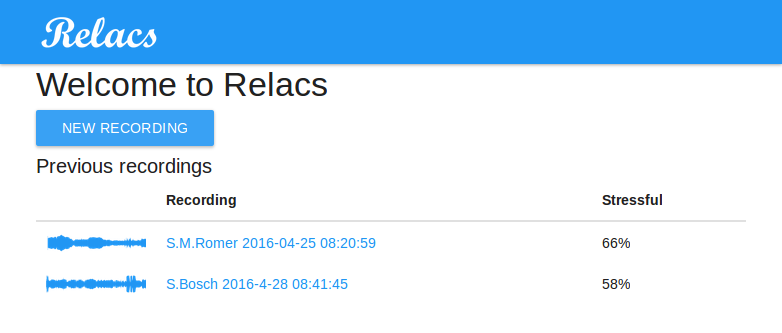
\includegraphics[width=0.9\linewidth]{./Website}
\caption{Screenshot of the overview page of the website, which contains previous recordings with previews of their respective .wav file, as well as the file name and the overall stress-level. At the current state of the project the `NEW RECORDING' button only acts as a place holder.}
\label{fig:Website}
\end{figure*}

\begin{figure*}[h]
\centering
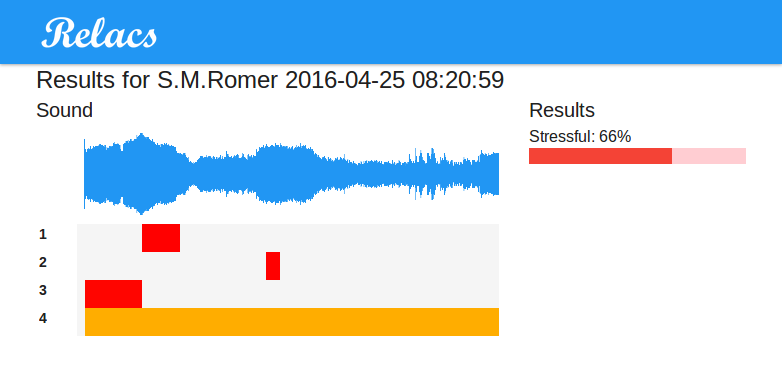
\includegraphics[width=0.9\linewidth]{./Audio1Results}
\caption{Screenshot of the results page of the website for one of the previous recordings. The results page contains the name of the recording as well as a visual representation of the .wav file. Underneath,  }
\label{fig:Audio1}
\end{figure*}

\begin{figure*}[h]
\centering
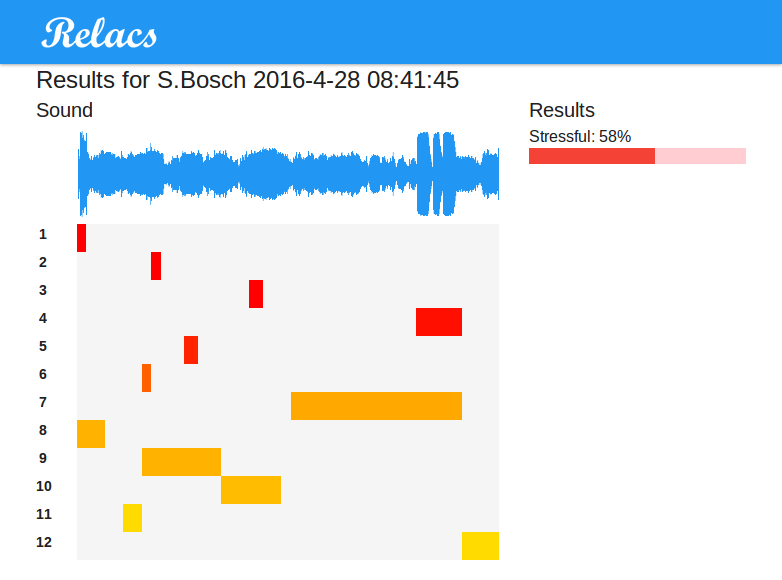
\includegraphics[width=0.9\linewidth]{./Audio2Results}
\label{fig:Audio2}
\end{figure*}

\section{Pitch sheets}

\begin{figure*}[h]
\centering
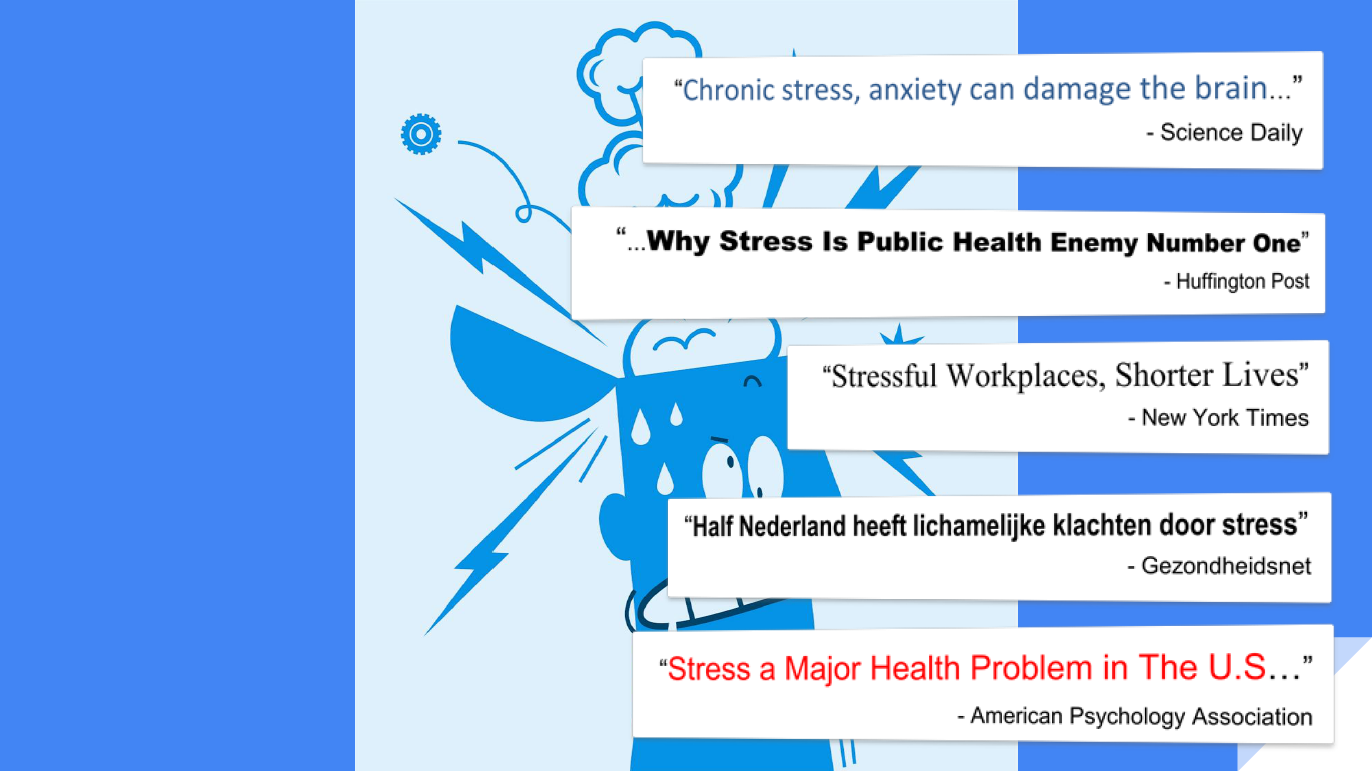
\includegraphics[width=\linewidth]{./Slide1}
\label{fig:Slide1}
\end{figure*}

\begin{figure*}[h]
\centering
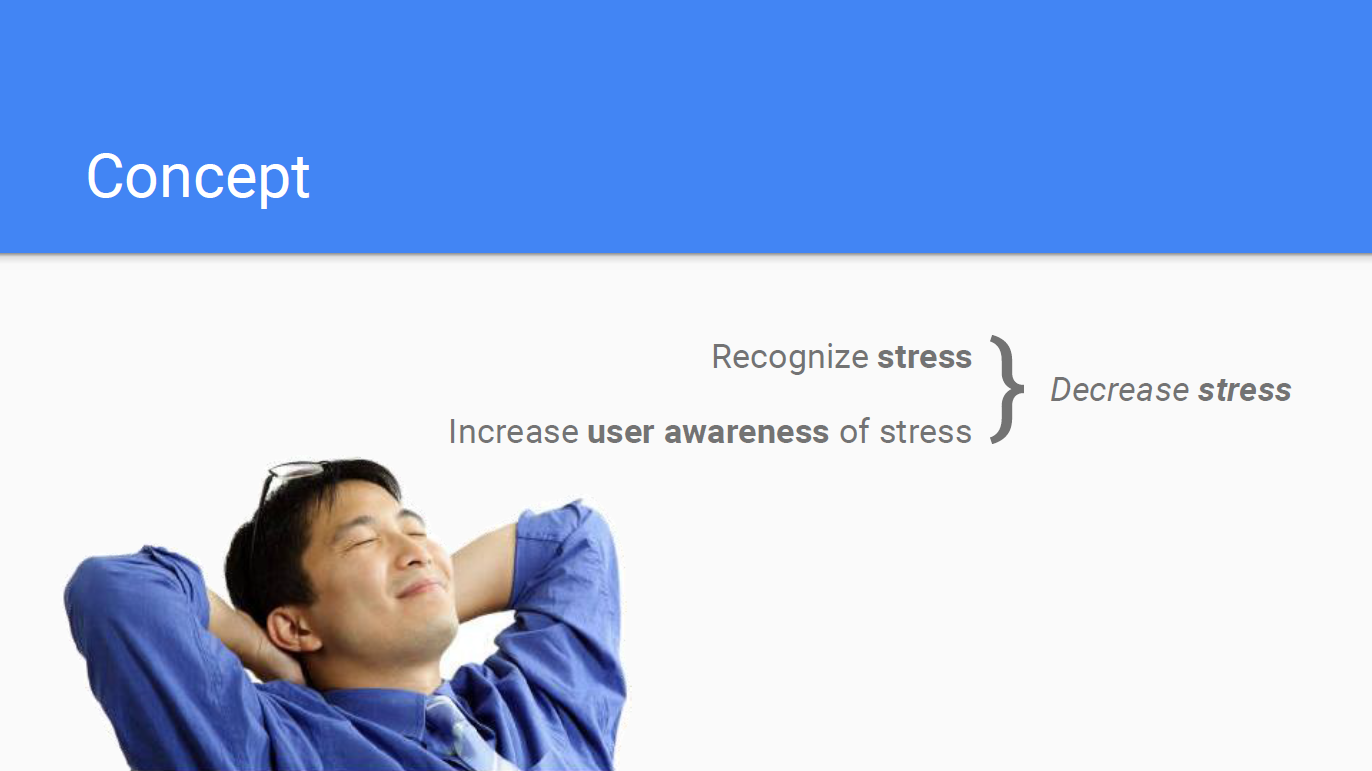
\includegraphics[width=\linewidth]{./Slide2}
\label{fig:Slide2}
\end{figure*}

\begin{figure*}[h]
\centering
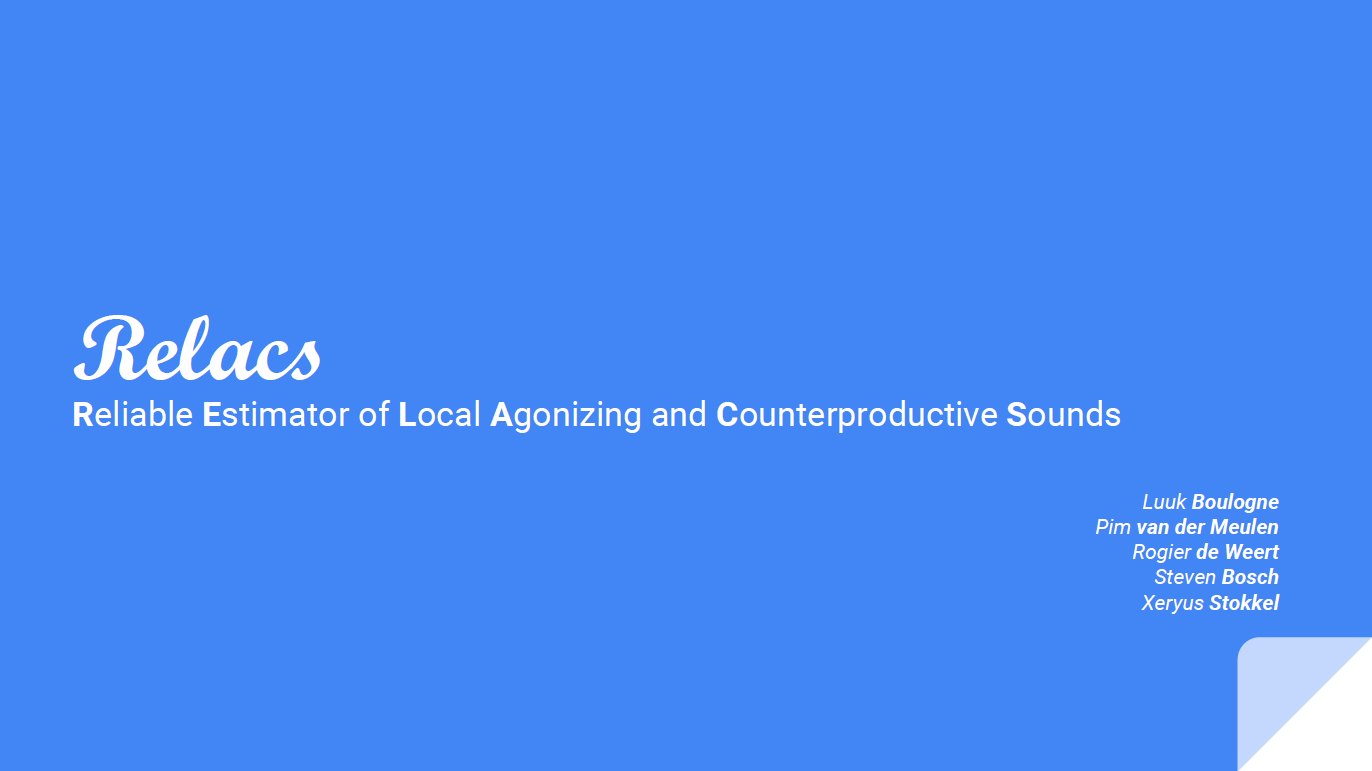
\includegraphics[width=\linewidth]{./Slide3}
\label{fig:Slide3}
\end{figure*}

\begin{figure*}[h]
\centering
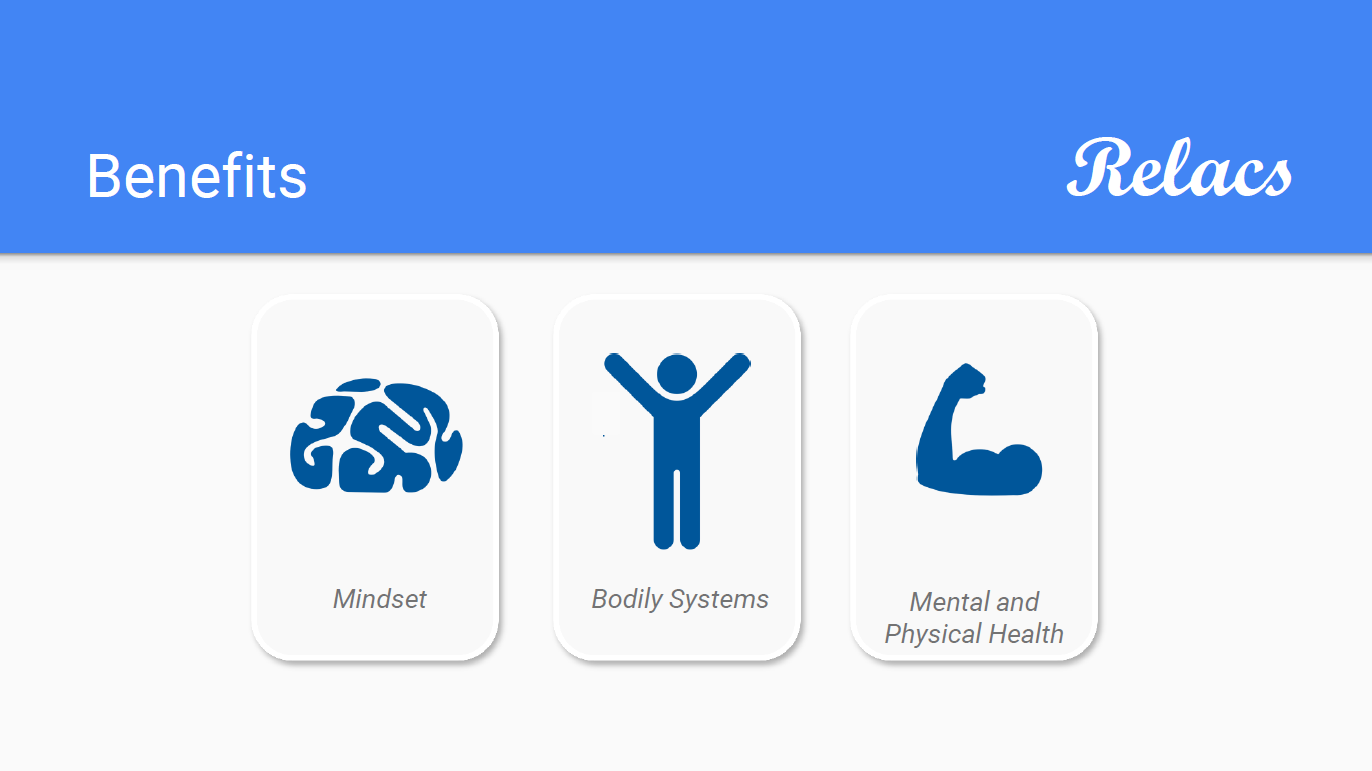
\includegraphics[width=\linewidth]{./Slide4}
\label{fig:Slide4}
\end{figure*}

\begin{figure*}[h]
\centering
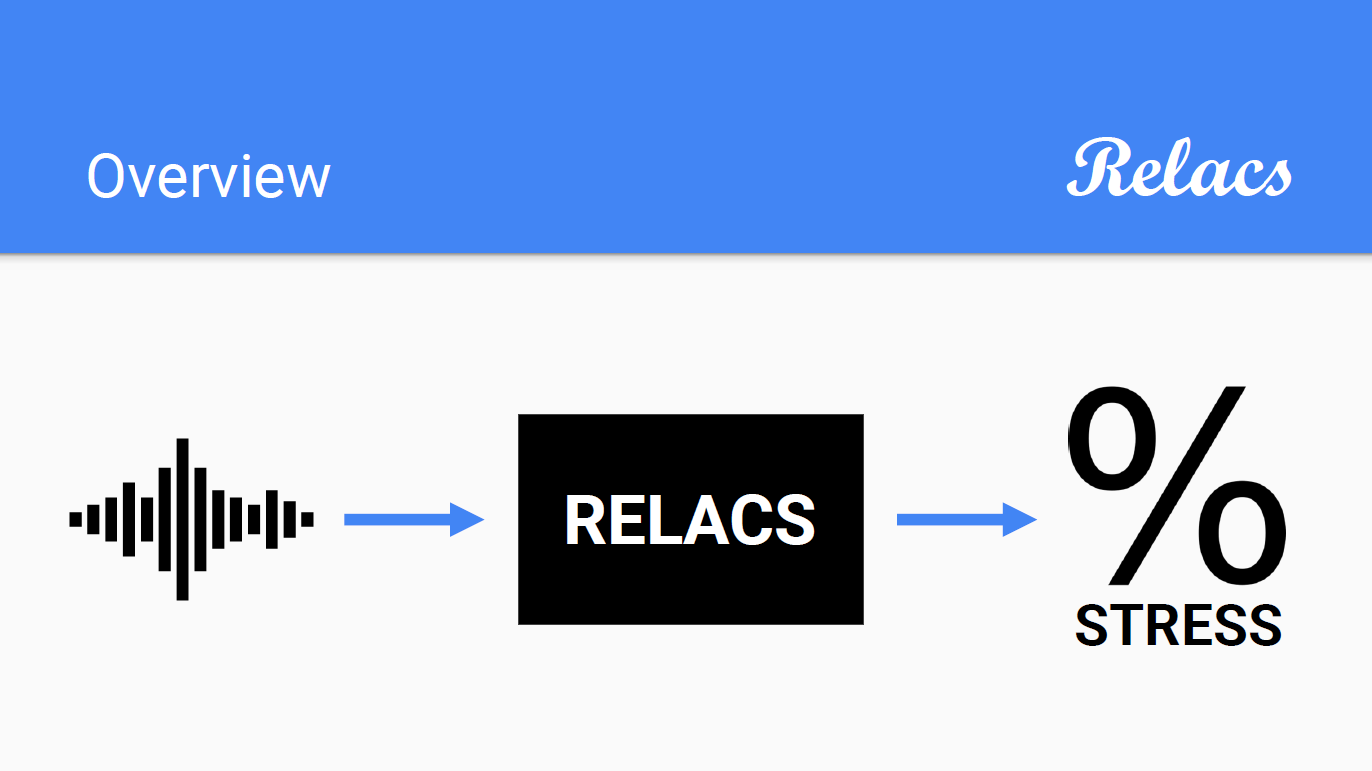
\includegraphics[width=\linewidth]{./Slide5}
\label{fig:Slide5}
\end{figure*}

\begin{figure*}[h]
\centering
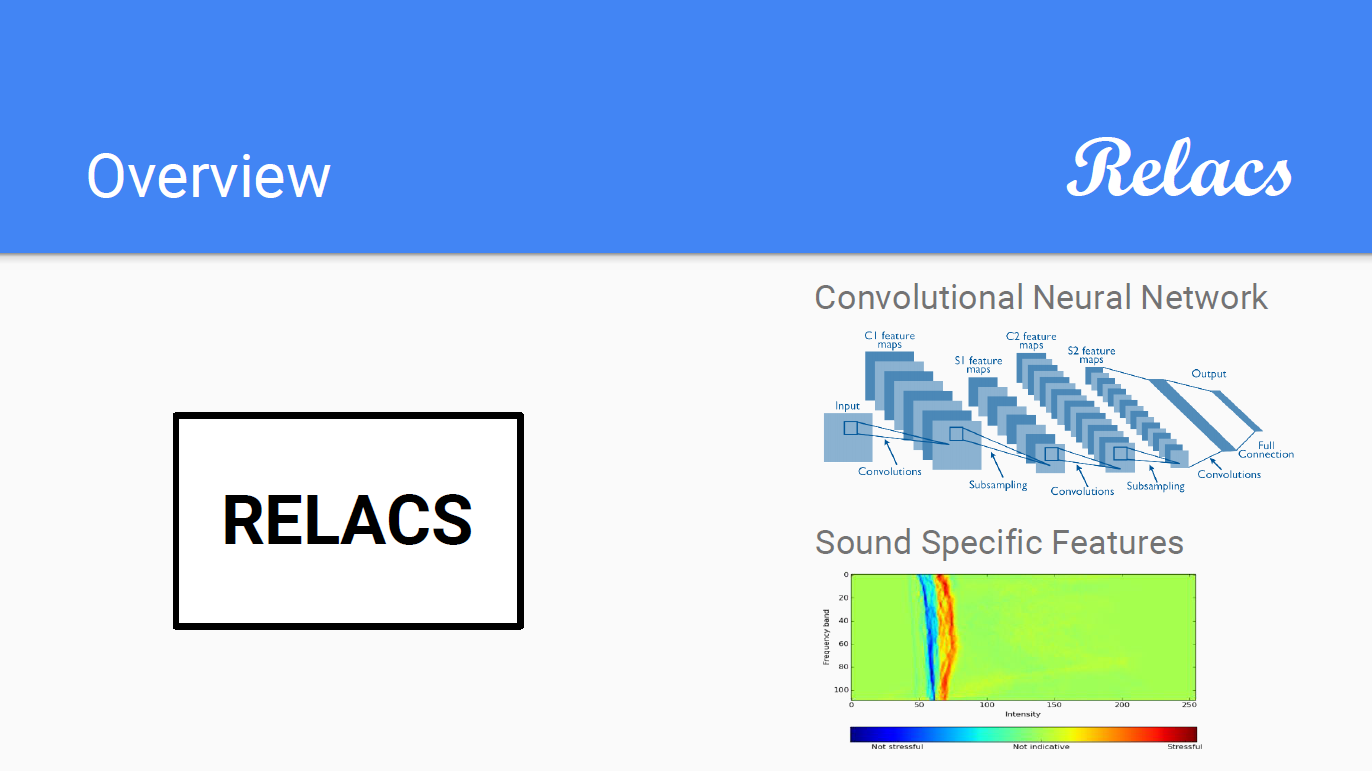
\includegraphics[width=\linewidth]{./Slide6}
\label{fig:Slide6}
\end{figure*}

\begin{figure*}[h]
\centering
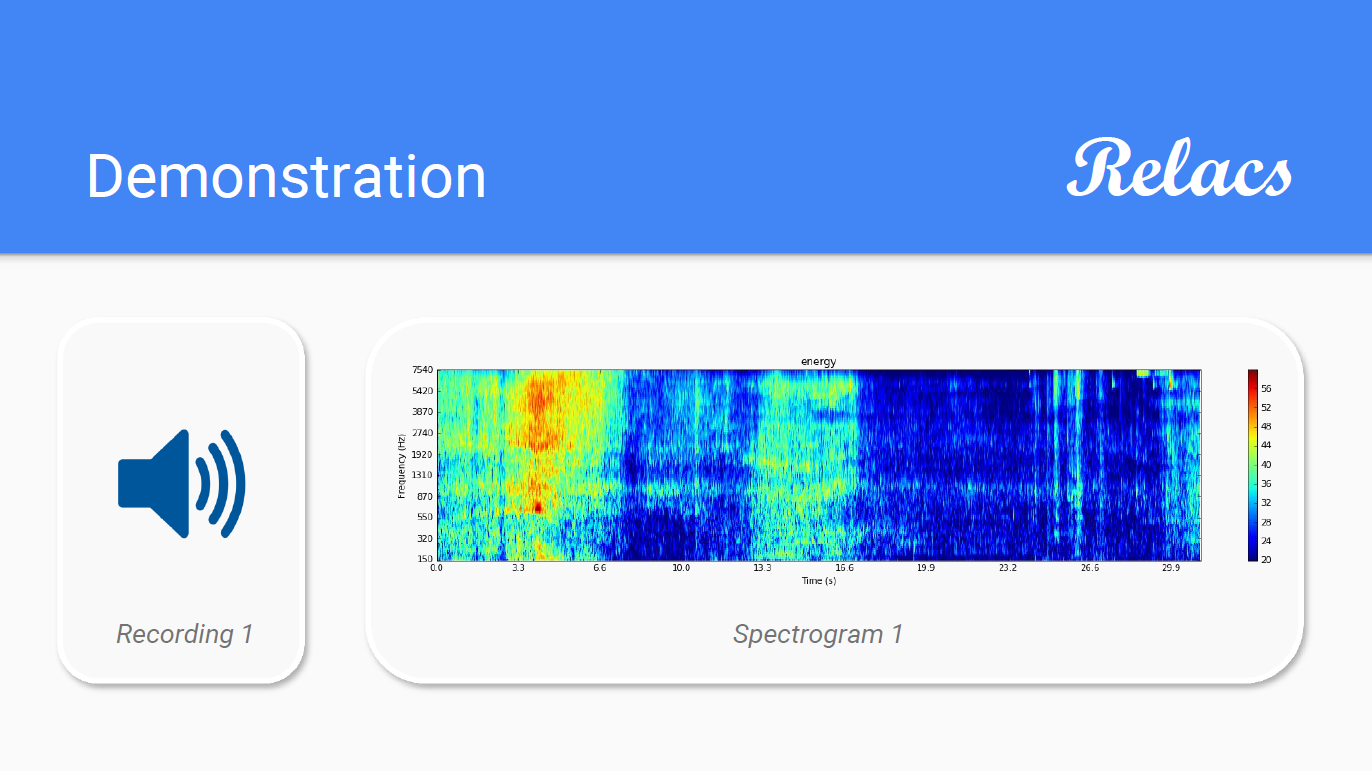
\includegraphics[width=\linewidth]{./Slide7}
\label{fig:Slide7}
\end{figure*}

\begin{figure*}[h]
\centering
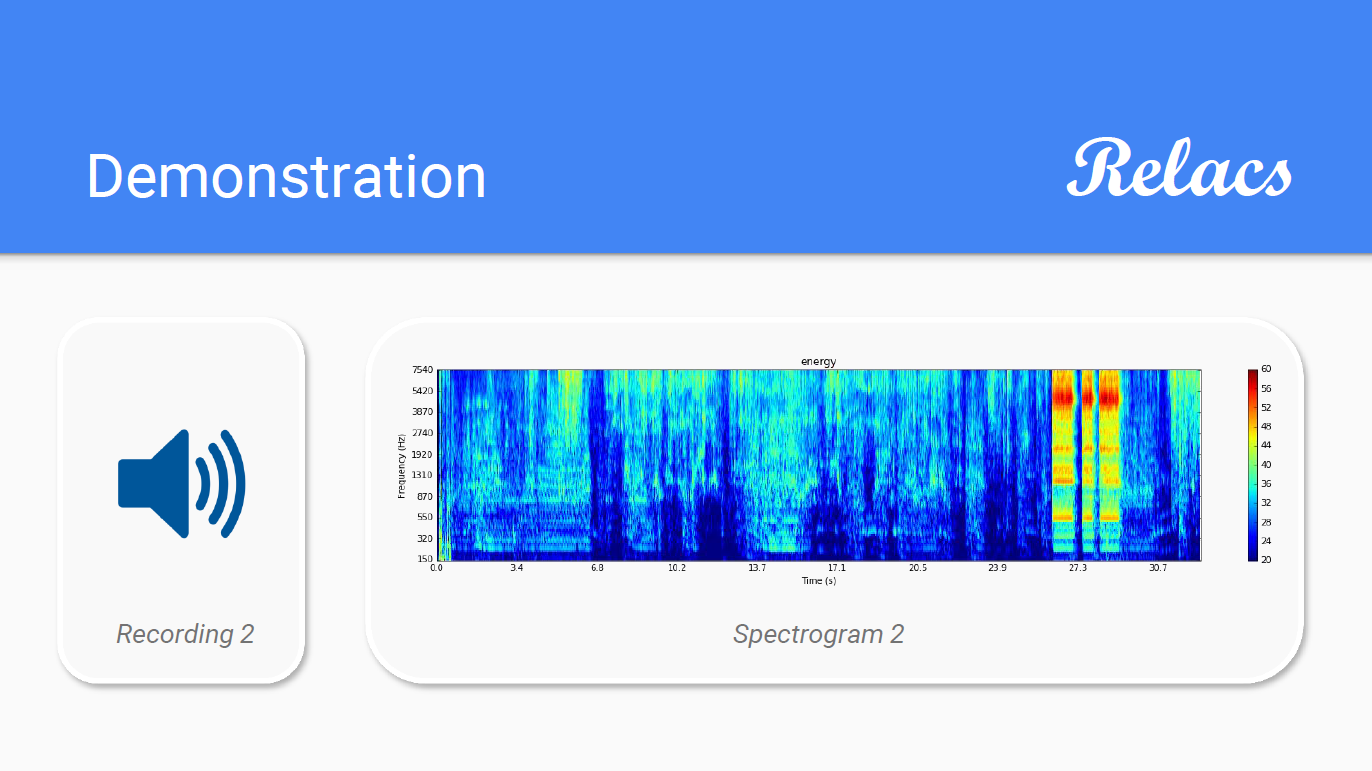
\includegraphics[width=\linewidth]{./Slide8}
\label{fig:Slide8}
\end{figure*}

\begin{figure*}[h]
\centering
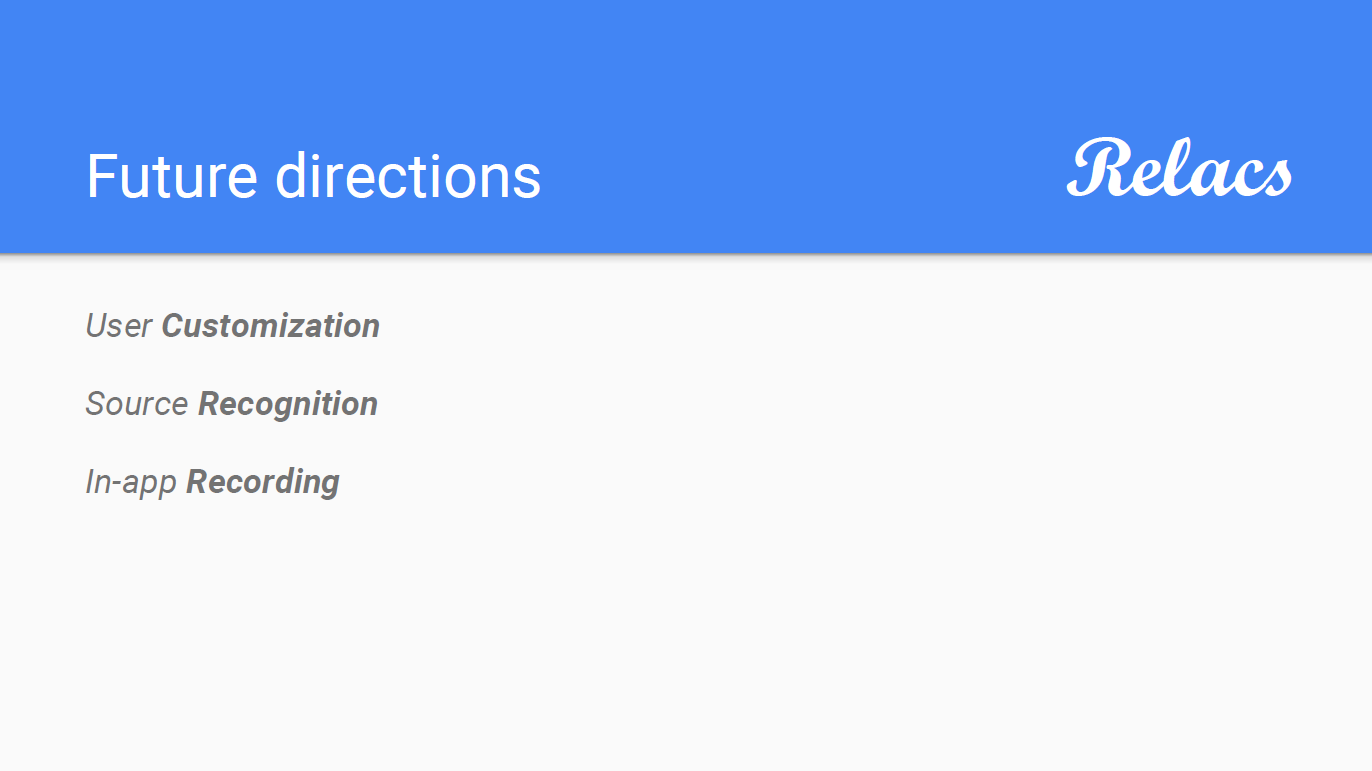
\includegraphics[width=\linewidth]{./Slide9}
\label{fig:Slide9}
\end{figure*}

\end{document}
